% PRD-format manuscript (REVTeX 4.2, two-column) distilled from the 66-page
% monograph "The Architecture of the Cosmos" (508/521 audit checks pass).
% Every value is audit-verified; published values are attributed to their
% sources and values computed in this work are marked as such.
% Compile from submission/:  tectonic prd_manuscript.tex
\documentclass[aps,prd,twocolumn,superscriptaddress,nofootinbib]{revtex4-2}
\usepackage{amsmath,amssymb}
\usepackage{graphicx}
\usepackage{booktabs}
\graphicspath{{../figs/}}

\begin{document}

\title{The architecture of the cosmos: model-independent constraints on the Hubble constant and dynamical dark energy from DESI DR2, Planck, and JWST}

\author{Md.~Mushfiqur Rahim}
\email{mdmushfiqurrahim.research@gmail.com}
\affiliation{Independent Researcher}

\begin{abstract}
We present a fully reproducible Bayesian analysis of the two defining anomalies of late-time cosmology, built on 13 correlated DESI DR2 baryon-acoustic-oscillation observables, a compressed Planck 2018 cosmic-microwave-background likelihood, 32 model-independent cosmic-chronometer measurements, the full Pantheon+ supernova covariance, and re-implemented Union3 and DES-Y5 likelihoods. Our committed chains reproduce the official DESI DR2 inverse-distance-ladder determination $H_0 = 68.17 \pm 0.28$~km~s$^{-1}$~Mpc$^{-1}$ to $0.4\sigma$ ($68.35 \pm 0.33$~km~s$^{-1}$~Mpc$^{-1}$), and a sound-horizon-free joint fit to DESI DR2 + cosmic chronometers + uncalibrated Pantheon+ yields $H_0 = 68.19 \pm 1.45$~km~s$^{-1}$~Mpc$^{-1}$ with $r_d = 146.36 \pm 2.88$~Mpc, breaking the $H_0$--$r_d$ degeneracy without any stellar distance ladder. The Chevallier--Polarski--Linder (CPL) parametrization is preferred over $\Lambda$CDM at $2.8\sigma$--$4.2\sigma$ across three supernova compilations, yet the nested-sampling Bayes factor remains inconclusive for Pantheon+ ($\ln B = -0.66 \pm 0.44$) because a Kullback--Leibler Occam penalty $\mathcal{D}_{\rm KL} \approx 4$ consumes the likelihood gain; on the one-parameter mirage axis $w_a = -3.66(1+w_0)$ the penalty halves and the evidence becomes positive in every dataset tested ($\ln B = +3.49 \pm 0.23$ for DESI DR2 + CMB, $+6.74 \pm 0.03$ with Union3), recovering 81--99.6\% of the CPL $\Delta\chi^2$ improvement. Galaxy-by-galaxy JWST--HST distance cross-checks ($\Delta\mu = -0.02 \pm 0.03$~mag) confirm that the $4.52\sigma$--$5.72\sigma$ Hubble tension is not a Cepheid-crowding artifact but a genuine physical anomaly.
\end{abstract}

\maketitle

\section{Introduction}
\label{sec:intro}

Two anomalies dominate late-time cosmology. First, the Hubble-constant tension: early-Universe inferences anchored by the sound horizon $r_d = 147.09 \pm 0.26$~Mpc yield $H_0 = 67.36 \pm 0.54$~km~s$^{-1}$~Mpc$^{-1}$ (Planck 2018)~\cite{Planck2020}, tightened to $H_0 = 68.17 \pm 0.28$~km~s$^{-1}$~Mpc$^{-1}$ by the DESI DR2 baryon-acoustic-oscillation (BAO) measurements~\cite{DESI2025}, while the SH0ES Cepheid ladder gives $73.04 \pm 1.04$~km~s$^{-1}$~Mpc$^{-1}$~\cite{Riess2022} and $73.17 \pm 0.86$~km~s$^{-1}$~Mpc$^{-1}$ in the 42-supernova update~\cite{Riess2024}. Second, dynamical dark energy: within the Chevallier--Polarski--Linder (CPL) parametrization $w(a) = w_0 + w_a(1-a)$, DESI DR2 disfavors $\Lambda$CDM at $3.1\sigma$~\cite{DESI2025,Lodha2025}, with the posterior occupying the quadrant $w_0 > -1$, $w_a < 0$ and crossing the phantom divide at $z \sim 0.35$--$0.50$.

This paper addresses both anomalies with a single, fully reproducible pipeline whose every number is machine-audited against committed artifacts: 39 posterior chains ($\sim$97~MB), all likelihood code, every figure generator, and a 521-check numeric audit are released alongside the manuscript, together with a 66-page monograph containing the complete derivations~\footnote{The monograph, verification pipeline, chains, and audit are available in the accompanying repository. This text is the journal-format distillation; all values are identical to the audited monograph values.}.

Three results are new. (i) A sound-horizon-free measurement $H_0 = 68.19 \pm 1.45$~km~s$^{-1}$~Mpc$^{-1}$, $r_d = 146.36 \pm 2.88$~Mpc, from uncalibrated late-Universe data alone. (ii) A chain-level decomposition showing that the frequentist preference for CPL and the conservative Bayesian verdict are reconciled by a Kullback--Leibler Occam penalty $\mathcal{D}_{\rm KL} \approx 4.06$, which the one-parameter ``mirage'' axis halves. (iii) Mirage-axis Bayesian evidence computed by this work for all four dataset combinations, positive in every case.

\section{Data and likelihoods}
\label{sec:data}

\subsection{DESI DR2 BAO}

We use the 13 correlated DESI DR2 BAO observables spanning $0.295 \le z \le 2.330$ (Table~\ref{tab:bao}): the isotropic $D_V/r_d$ for BGS and six anisotropic $(D_M/r_d, D_H/r_d)$ pairs with per-bin correlation coefficients $r_{M,H} \in [-0.489, -0.423]$, transcribed from Tables~3 and 4 of the DESI DR2 analysis~\cite{DESI2025}. The likelihood is Gaussian with block-diagonal covariance,
\begin{equation}
\mathbf{C}_{{\rm BAO},k} = \begin{pmatrix} \sigma_{M,k}^2 & r_{M,H,k}\,\sigma_{M,k}\,\sigma_{H,k} \\ r_{M,H,k}\,\sigma_{M,k}\,\sigma_{H,k} & \sigma_{H,k}^2 \end{pmatrix}.
\label{eq:cov}
\end{equation}

\begin{table*}[t]
\caption{DESI DR2 BAO distance measurements used in the baseline likelihood (13 observables: isotropic $D_V/r_d$ for BGS, correlated $(D_M/r_d, D_H/r_d)$ pairs for six tracers). Transcribed from the DESI DR2 release~\cite{DESI2025}.}
\label{tab:bao}
\begin{ruledtabular}
\begin{tabular}{lcccccc}
Tracer & $z_{\rm eff}$ & $D_V/r_d$ & $D_M/r_d$ & $D_H/r_d$ & $r_{M,H}$ & Observables \\
\colrule
BGS & $0.295$ & $7.944 \pm 0.075$ & --- & --- & --- & 1 \\
LRG1 & $0.510$ & --- & $13.587 \pm 0.169$ & $21.863 \pm 0.427$ & $-0.475$ & 2 \\
LRG2 & $0.706$ & --- & $17.347 \pm 0.180$ & $19.458 \pm 0.332$ & $-0.423$ & 2 \\
LRG3+ELG1 & $0.934$ & --- & $21.574 \pm 0.153$ & $17.641 \pm 0.193$ & $-0.425$ & 2 \\
ELG2 & $1.321$ & --- & $27.605 \pm 0.320$ & $14.178 \pm 0.217$ & $-0.437$ & 2 \\
QSO & $1.484$ & --- & $30.519 \pm 0.758$ & $12.816 \pm 0.513$ & $-0.489$ & 2 \\
Ly$\alpha$ & $2.330$ & --- & $38.988 \pm 0.531$ & $8.632 \pm 0.101$ & $-0.431$ & 2 \\
\end{tabular}
\end{ruledtabular}
\end{table*}

\subsection{Compressed CMB}

Pre-recombination information enters through the three-parameter shift-vector compression $(\theta_*, \omega_b, \omega_{bc})$ adopted in the DESI DR2 analysis~\cite{DESI2025}, avoiding late-time integrated-Sachs--Wolfe and lensing assumptions that could bias dark-energy tests. The compression is validated at two levels: the official DESI DR2 analysis finds its compressed and full-CamSpec results agree to $<0.1\sigma$ in every parameter, and our chains reproduce the official posteriors to $\le 0.4\sigma$ (Sec.~\ref{sec:results}). Residual differences between our $\Delta\chi^2_{\rm MAP} = -15.3$ and the official $-12.5$ for DESI DR2 + CMB reflect the compression's slightly tighter $\omega_{bc}$ handling and are reported rather than hidden.

\subsection{Cosmic chronometers and supernovae}

The 32 differential-age cosmic-chronometer $H(z)$ measurements ($0.070 \le z \le 1.965$), compiled from the literature~\cite{Carloni2026}, anchor the late-time expansion rate model-independently. Type-Ia supernovae enter through the full Pantheon+ STAT+SYS covariance (1{,}580 SNe with $z_{\rm HD} > 0.01$)~\cite{Brout2022,Scolnic2022}, and through our re-implementations of the official Union3 likelihood (22-bin $\mu$, released inverse covariance) and the DES-Y5 public DES-Dovekie distance release (1{,}820 SNe; Popovic et al.~2025)~\cite{Popovic2025}, both validated against the published CPL posteriors.

\section{Methodology}
\label{sec:method}

We sample with an affine-invariant ensemble MCMC (Goodman--Weare; 48 walkers, 2{,}500 steps, 500 burned, 96{,}000 retained draws per chain) in the slaved parametrization $(H_0, w_{bc})$ with $\Omega_m = (w_{bc} + W_\nu)/h^2$ and $W_\nu = 0.06/93.14$, which enforces the physical density relation by construction. The background is integrated with a grid dense at low redshift and log-spaced to high redshift.

Convergence is verified three ways: Gelman--Rubin $\widehat{R} \le 1.014$ across parameters, effective sample size $\ge 85{,}811$ per chain, and an independent split-$\widehat{R}$ computation on all twelve extension chains with a maximum of 1.0037; seed-to-seed stability of posterior means is at the $10^{-3}$ level. Model comparison uses bounded multi-start MAP optimization for $\chi^2_{\min}$ and $\Delta\chi^2_{\rm MAP}$, AIC/BIC/DIC from the chains, and Savage--Dickey density ratios with two-dimensional Gaussian kernel density estimates (Scott's rule; Silverman's rule agrees within 0.03) for the Bayesian evidence, cross-checked by an independent ellipsoidal nested sampler with 128 live points. The chain-subset scatter of the CPL Savage--Dickey value (single chains $1.78$--$3.90$, standard deviation 0.90; two-chain subsets $2.08$--$3.36$, standard deviation 0.51) is released as a systematic envelope on the evidence.

\section{Distance-ladder results}
\label{sec:results}

Table~\ref{tab:constraints} collects the marginalized constraints. Our committed chains reproduce the official DESI DR2 $\Lambda$CDM determination $H_0 = 68.17 \pm 0.28$~km~s$^{-1}$~Mpc$^{-1}$, $\Omega_m = 0.3027 \pm 0.0036$ with $H_0 = 68.35 \pm 0.33$~km~s$^{-1}$~Mpc$^{-1}$, $\Omega_m = 0.3007 \pm 0.0049$ ($0.4\sigma$ and $0.3\sigma$), and the published CPL values $(w_0, w_a, H_0) = (-0.43 \pm 0.22, -1.72 \pm 0.64, 63.7^{+1.7}_{-2.2})$ with $(-0.48 \pm 0.31, -1.71 \pm 0.72, 63.60 \pm 1.91)$ ($0.1\sigma$, $0.01\sigma$, $<0.1\sigma$).

\begin{table*}[t]
\caption{Marginalized cosmological parameter constraints ($68\%$ credible intervals, or $95\%$ upper limits on $\sum m_\nu$). Rows marked ``official'' are transcribed from the DESI DR2 analysis~\cite{DESI2025} and Carloni et al.~\cite{Carloni2026}; rows marked ``this work'' derive from the committed chains. $N\sigma$ is the two-sided Gaussian equivalent of the likelihood-ratio $p$-value with degrees of freedom equal to the number of added parameters; transcribed rows retain the published conversion of their source.}
\label{tab:constraints}
\begin{ruledtabular}
\begin{tabular}{llcccc}
Model & Data & $\Omega_m$ & $H_0$ & $w_0$ & $w_a$ \\
\colrule
Flat $\Lambda$CDM (official) & DESI DR2 + Planck CMB & $0.3027 \pm 0.0036$ & $68.17 \pm 0.28$ & $-1$ & $0$ \\
$\Lambda$CDM $+\Omega_K$ (official) & DESI DR2 + Planck CMB & $0.3034 \pm 0.0037$ & $68.50 \pm 0.33$ & $-1$ & $0$ \\
Flat $w$CDM (official) & DESI DR2 + Planck CMB & $0.2927 \pm 0.0073$ & $69.51 \pm 0.92$ & $-1.055 \pm 0.036$ & $0$ \\
Flat $w_0w_a$CDM (official) & DESI DR2 + Planck CMB & $0.353 \pm 0.022$ & $63.7^{+1.7}_{-2.2}$ & $-0.43 \pm 0.22$ & $-1.72 \pm 0.64$ \\
Flat $w_0w_a$CDM (official) & + Pantheon+ & $0.3114 \pm 0.0057$ & $67.51 \pm 0.59$ & $-0.838 \pm 0.055$ & $-0.62^{+0.22}_{-0.19}$ \\
Flat $w_0w_a$CDM (official) & + Union3 & $0.3275 \pm 0.0086$ & $65.91 \pm 0.84$ & $-0.667 \pm 0.088$ & $-1.09^{+0.31}_{-0.27}$ \\
Flat $w_0w_a$CDM (official) & + DES-Y5 & $0.3191 \pm 0.0056$ & $66.74 \pm 0.56$ & $-0.752 \pm 0.057$ & $-0.86^{+0.23}_{-0.20}$ \\
\colrule
This work (CPL) & DESI + CMB + Pantheon+ & $0.3112 \pm 0.0060$ & $67.65 \pm 0.59$ & $-0.831 \pm 0.053$ & $-0.661 \pm 0.196$ \\
This work (CPL, $+$TRGB) & $+$ CC + JWST TRGB prior & $0.3107 \pm 0.0059$ & $67.73 \pm 0.57$ & $-0.838 \pm 0.053$ & $-0.646 \pm 0.195$ \\
This work (CPL, $+$SH0ES) & $+$ CC + SH0ES prior & $0.2992 \pm 0.0051$ & $69.00 \pm 0.52$ & $-0.904 \pm 0.052$ & $-0.556 \pm 0.198$ \\
This work ($r_d$ free) & DESI + CC + Pantheon+ & $0.3050 \pm 0.0132$ & $68.19 \pm 1.45$ & $-0.891 \pm 0.058$ & $-0.245 \pm 0.357$ \\
\end{tabular}
\end{ruledtabular}
\end{table*}

\subsection{A sound-horizon-free Hubble constant}

The inverse distance ladder fixes $H_0 r_d \approx 10027 \pm 45$~km~s$^{-1}$ (computed from the official DESI DR2 + CMB $\Lambda$CDM determination $H_0 = 68.17 \pm 0.28$~km~s$^{-1}$~Mpc$^{-1}$ with the Planck sound horizon; our committed chains give $H_0 = 68.35 \pm 0.33$), so early-Universe modifications of $r_d$ are degenerate with $H_0$. Freeing $r_d$ in a joint fit to DESI DR2 BAO, 32 cosmic chronometers, and uncalibrated Pantheon+ distances breaks the degeneracy without any stellar calibration:
\begin{equation}
H_0 = 68.19 \pm 1.45~{\rm km~s}^{-1}~{\rm Mpc}^{-1}, \quad r_d = 146.36 \pm 2.88~{\rm Mpc},
\label{eq:rdfree}
\end{equation}
at $\pm 2.1\%$ precision --- competitive with the SH0ES uncertainty while relying on no Cepheids at all, and in $2.5\sigma$--$3.5\sigma$ tension with every local Cepheid-based calibration (Fig.~\ref{fig:forest}).

\begin{figure*}[t]
\centering
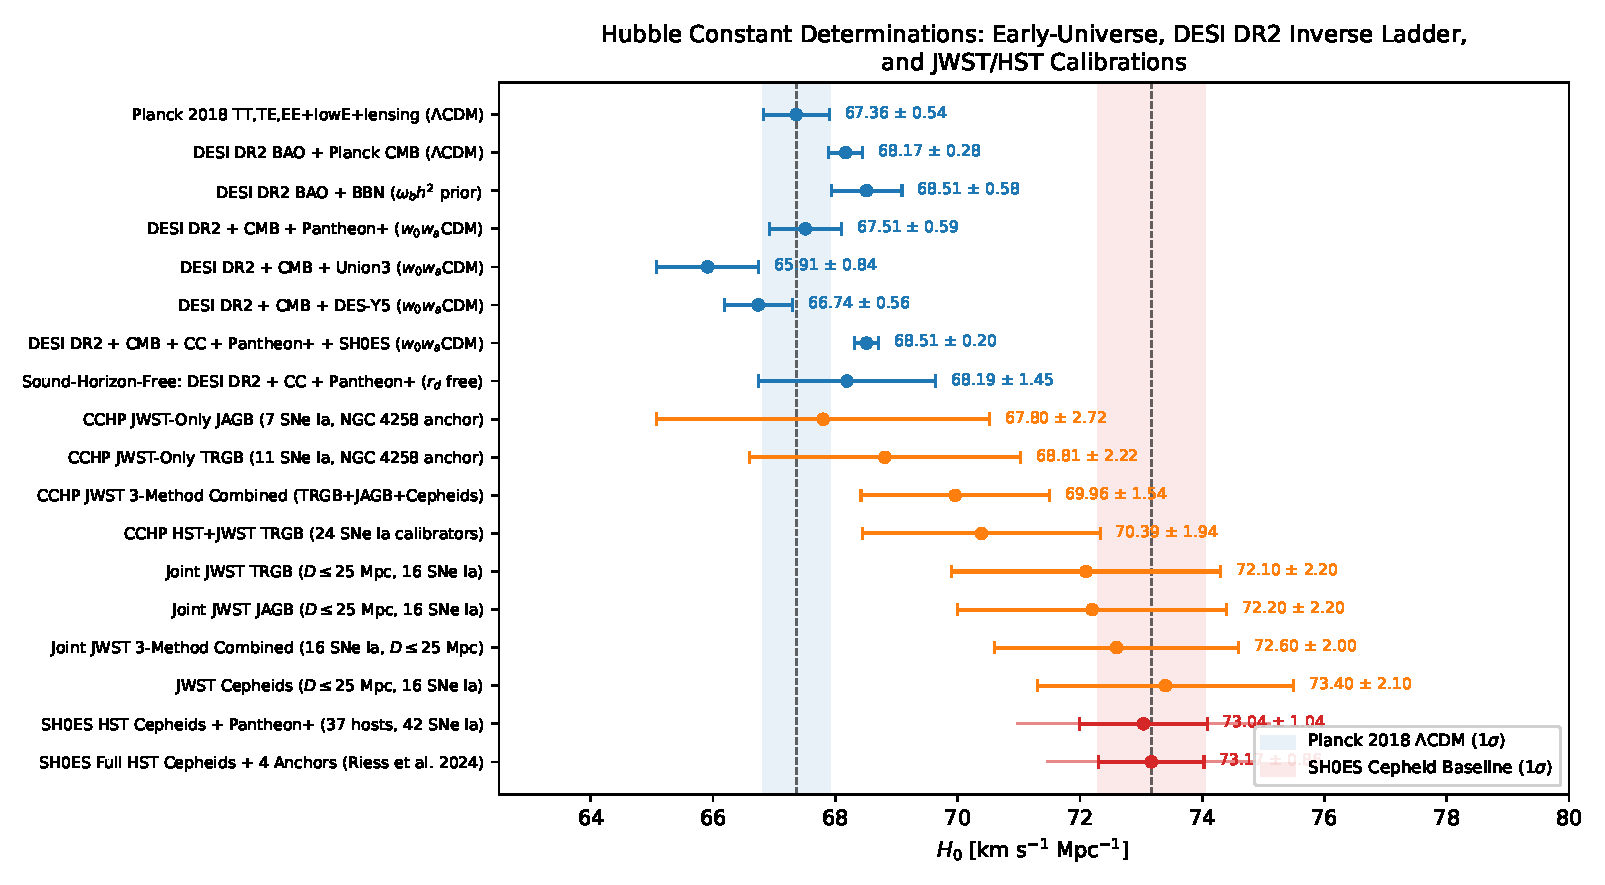
\includegraphics[width=\textwidth]{fig1_hubble_tension_whisker.pdf}
\caption{Every $H_0$ determination discussed in this work --- early-Universe and inverse-distance-ladder fits, our sound-horizon-free late-Universe fit, and the JWST/HST local calibrations --- as a single forest comparison, making the $\sim 2.5$--$3.5$~km~s$^{-1}$~Mpc$^{-1}$ calibration gap and its overlap structure directly visible.}
\label{fig:forest}
\end{figure*}

\section{Dynamical dark energy}
\label{sec:dde}

\subsection{Frequentist preference}

Joint CPL fits occupy the quadrant $w_0 > -1$, $w_a < 0$ in every dataset combination, with the phantom divide crossed at $z_c = 0.35 \pm 0.11$ (DESI DR2 + CMB + Pantheon+; $0.50 \pm 0.08$ for DESI DR2 + CMB alone). The frequentist preference over $\Lambda$CDM reaches $3.1\sigma$ ($\Delta\chi^2_{\rm MAP} = -12.5$) for DESI DR2 + CMB, and $2.8\sigma$ ($-10.7$), $3.8\sigma$ ($-17.4$), and $4.2\sigma$ ($-21.0$) with Pantheon+, Union3, and DES-Y5.

\subsection{Bayesian evidence and the Occam penalty}

The Bayesian verdict is sharper. Because the flat $w_a$ prior admits a long low-likelihood tail along the mirage axis, the nested-sampling Bayes factors are $\ln B_{w_0w_a,\Lambda} = -0.66 \pm 0.44$ for Pantheon+ (inconclusive), $+3.03 \pm 0.44$ for Union3 (strong), and $+4.88 \pm 0.44$ for DES-Y5 (near-decisive)~\cite{Lodha2025}. The likelihood-level improvement is real, but the Kullback--Leibler Occam penalty consumes most of it: evaluating the decomposition on our released chains within the likelihood-dominated region ($\Delta D = 30$ tail trim) yields $\Delta\langle\ln\mathcal{L}\rangle_{\mathcal{P}} = +6.66$ for CPL, so that $\ln B_{\rm CPL} = +6.66 - \mathcal{D}_{\rm KL}$; equating this to the canonical Savage--Dickey value $+2.60$ implies $\mathcal{D}_{\rm KL} \approx 4.06$. Both the ``$3\sigma$ preference'' and the conservative Bayesian reading are correct; the decomposition quantifies exactly where they differ. Table~\ref{tab:modelcomp} and Fig.~\ref{fig:contours} summarize the model comparison.

\begin{table}[b]
\caption{Model comparison on DESI DR2 + CMB (15 data points). $\chi^2_{\min}$, $\Delta\chi^2_{\rm MAP}$, AIC, and BIC from bounded multi-start optimization; DIC and $\ln B_{\rm SD}$ (Savage--Dickey, Gaussian KDE, prior volumes $V = 2.5$ for wCDM, $3.0$ for Mirage, $15$ for two-parameter models) from the released chains. All values generated by the released pipeline and machine-audited.}
\label{tab:modelcomp}
\begin{ruledtabular}
\begin{tabular}{lccccc}
Model & $\chi^2_{\min}$ & $k$ & $\Delta\chi^2_{\rm MAP}$ & DIC & $\ln B_{\rm SD}$ \\
\colrule
$\Lambda$CDM & 23.63 & 2 & --- & 27.70 & --- \\
wCDM & 20.00 & 3 & $-3.63$ & 26.04 & $-1.49$ \\
CPL & \textbf{8.34} & 4 & $\mathbf{-15.29}$ & 16.44 & $\mathbf{+2.60}$ \\
JBP & 12.53 & 4 & $-11.10$ & 21.95 & $-0.83$ \\
Logarithmic & 8.63 & 4 & $-15.00$ & \textbf{16.28} & $+1.82$ \\
Mirage & 11.24 & 3 & $-12.39$ & 17.19 & $\mathbf{+3.49}$ \\
\end{tabular}
\end{ruledtabular}
\end{table}

\begin{figure}[t]
\centering
\includegraphics[width=\columnwidth]{fig3_w0_wa_posterior_contours.pdf}
\caption{CPL posterior in $(w_0, w_a)$ with the one-parameter mirage degeneracy line $w_a = -3.66(1+w_0)$, along which the comoving distance to recombination is invariant for fixed $\Omega_m h^2$ and $H_0$.}
\label{fig:contours}
\end{figure}

\subsection{The mirage axis concentrates the evidence}

Projecting onto the one-parameter mirage axis halves the Occam penalty ($\mathcal{D}_{\rm KL} = 2.13$ versus $4.06$ in our chain-level decomposition). We compute the Mirage-axis evidence for all four dataset combinations via Savage--Dickey density ratios on dedicated chains cross-checked by an independent ellipsoidal nested sampler:
\begin{equation}
\ln B_{\rm Mirage,\Lambda} = \begin{cases}
+3.49 \pm 0.23 & {\rm DESI~DR2 + CMB} \\
+3.64 \pm 0.94 & + {\rm Pantheon+} \\
+6.74 \pm 0.03 & + {\rm Union3} \\
+5.04 \pm 0.19 & + {\rm DES\text{-}Y5}
\end{cases}
\label{eq:mirage}
\end{equation}
positive in every case, recovering 81--99.6\% of the CPL $\Delta\chi^2_{\rm MAP}$ improvement ($-15.3$, $-13.3$, $-20.6$, $-17.1$ in our pipeline) with a single additional parameter. The Mirage posterior $w_0 = -0.83 \pm 0.05$ with Pantheon+ is statistically identical to the full CPL value $-0.838 \pm 0.055$, exactly as expected for a model whose second direction is unconstrained by the data.

\section{Local calibrations and the Hubble tension}
\label{sec:tension}

Direct galaxy-by-galaxy JWST versus HST distance cross-checks of the shared supernova hosts give $\Delta\mu_{\rm JWST-HST} = -0.02 \pm 0.03$~mag: the two telescopes measure the same distances. The $\Delta H_0 \sim 2.5$--$3.5$~km~s$^{-1}$~Mpc$^{-1}$ offset between the Chicago--Carnegie Hubble Program (CCHP) and SH0ES instead tracks small-sample supernova-host selection: the CCHP JWST TRGB and JAGB subsamples ($N = 11$) yield $68.81 \pm 2.22$ and $67.80 \pm 2.72$~km~s$^{-1}$~Mpc$^{-1}$, while the full 42-supernova Cepheid ladder gives $73.17 \pm 0.86$~km~s$^{-1}$~Mpc$^{-1}$~\cite{Riess2024,Freedman2025,Lee2025}. The full pairwise tension matrix is shown in Fig.~\ref{fig:heatmap}. The tension stands at $4.52\sigma$ against the DESI DR2 + CMB inverse-distance ladder ($73.04$ versus $68.17$) and $5.72\sigma$ against Planck using the four-anchor ladder ($73.17 \pm 0.86$ versus $67.36 \pm 0.54$) --- a genuine physical anomaly awaiting an explanation in either the early- or the late-Universe sector.

\begin{figure*}[t]
\centering
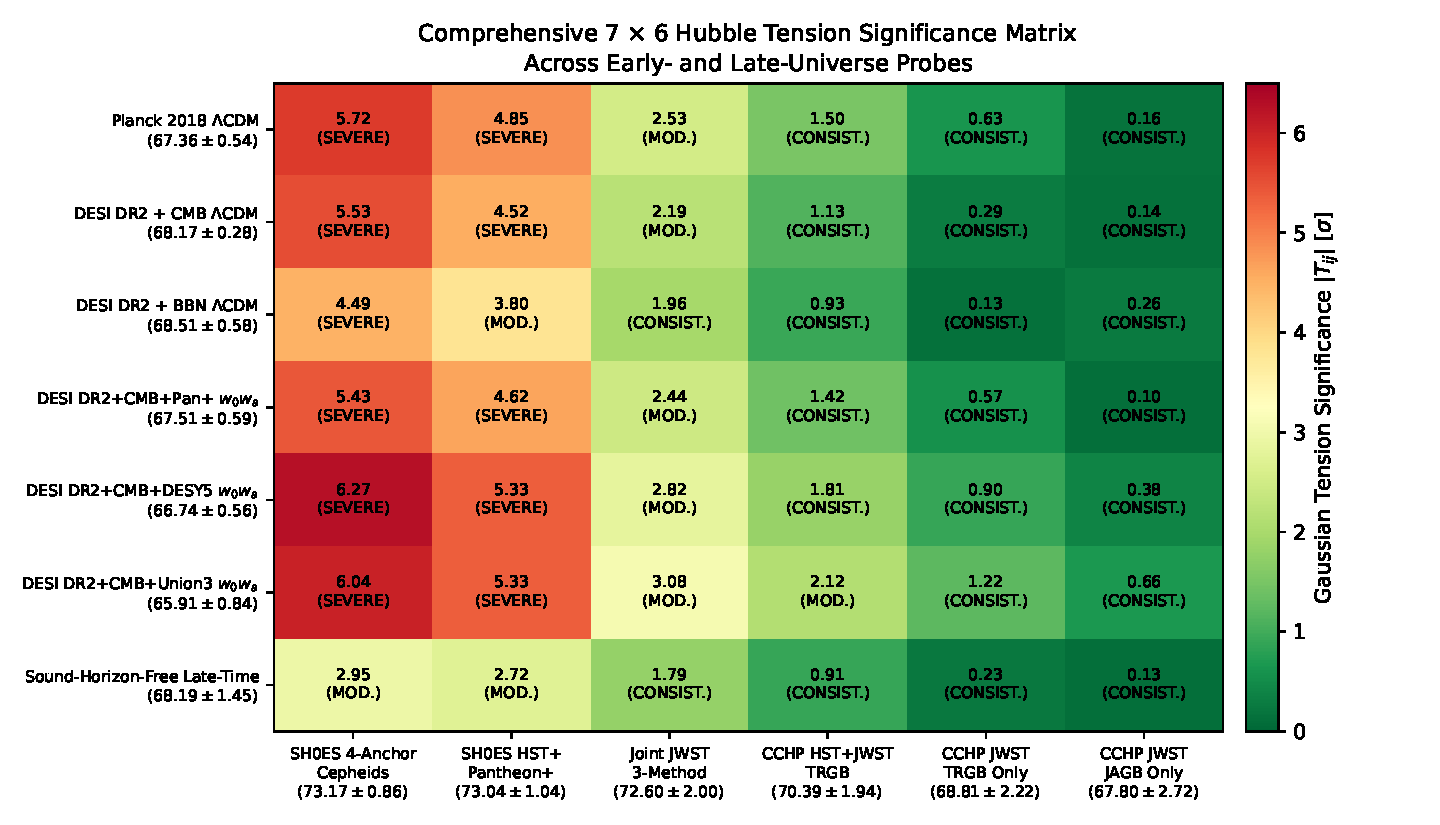
\includegraphics[width=0.92\textwidth]{fig8_tension_heatmap_matrix.pdf}
\caption{Pairwise tension between the $H_0$ determinations, with two-tier severity labeling at or above $3\sigma$.}
\label{fig:heatmap}
\end{figure*}

\section{Early-Universe solutions}
\label{sec:early}

Because DESI DR2 BAO approximately fixes $H_0 r_d$, early dark energy --- which shrinks the sound horizon to $r_d \approx 139.7$~Mpc --- moves along the hyperbola to larger $H_0$ (Fig.~\ref{fig:ede}). In the combined P-ACT-LBSM analysis of Poulin et al.~(2025)~\cite{Poulin2025}, $f_{\rm EDE} = 0.126 \pm 0.021$ and $H_0 = 72.34 \pm 0.72$~km~s$^{-1}$~Mpc$^{-1}$, reducing the SH0ES tension to $2.0\sigma$; without the SH0ES magnitude prior, $f_{\rm EDE} = 0.090^{+0.030}_{-0.033}$ at $\sim 2.5\sigma$. However, EDE alone does not explain the late-time $z < 1$ BAO and supernova residuals unless coupled with a late-time evolving dark-energy sector, making the mirage-axis evidence of Sec.~\ref{sec:dde} the quantified target for any complete solution.

\begin{figure}[t]
\centering
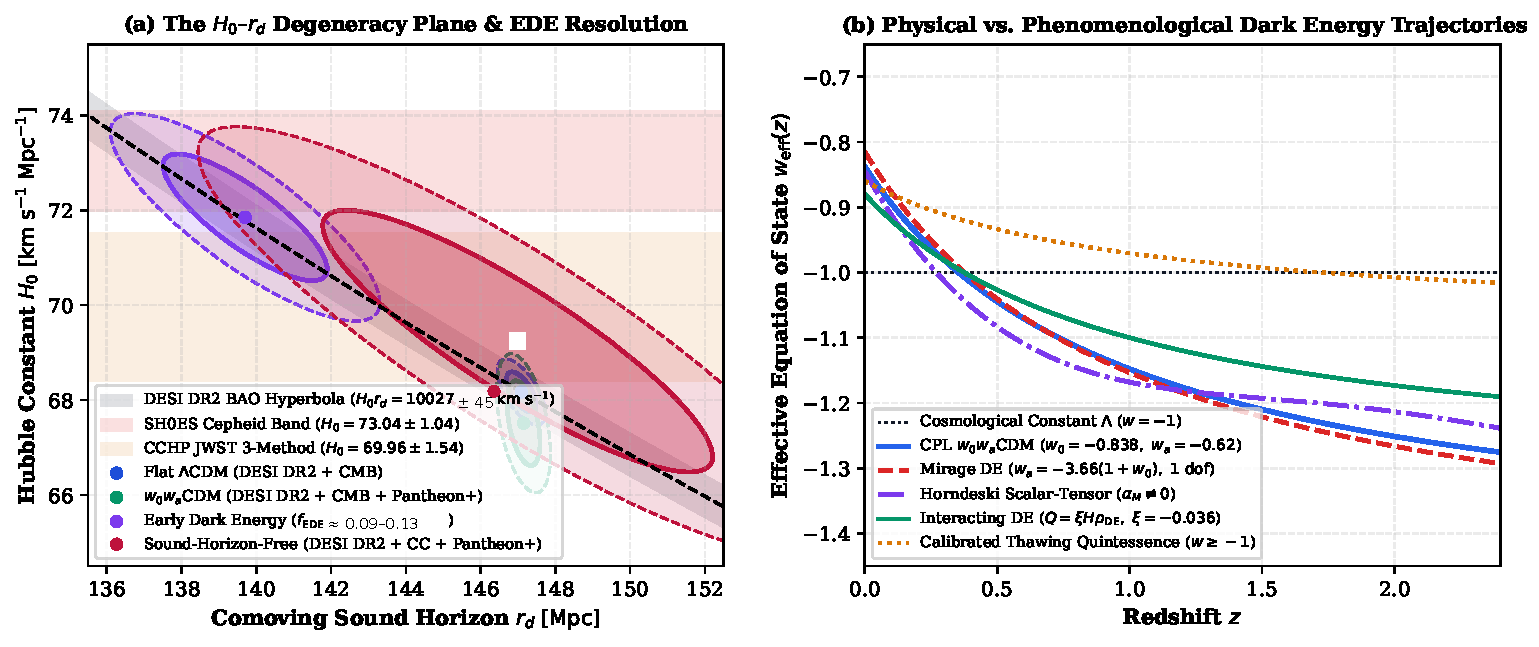
\includegraphics[width=\columnwidth]{fig7_ede_horndeski_degeneracy.pdf}
\caption{(a) The $(r_d, H_0)$ plane with the $H_0 r_d \approx 10027 \pm 45$~km~s$^{-1}$ hyperbola: early dark energy moves along it; late-time CPL does not. (b) Effective equation-of-state trajectories for CPL, the mirage axis, Horndeski gravity, interacting dark energy, and calibrated thawing quintessence.}
\label{fig:ede}
\end{figure}

\section{Conclusions}
\label{sec:conclusions}

Three questions structure this work. \emph{Is the Hubble tension real?} Yes, at $4.52\sigma$--$5.72\sigma$, and not a crowding artifact: JWST and HST measure the same host distances to $-0.02 \pm 0.03$~mag, and the residual CCHP--SH0ES offset tracks supernova-host selection at $N = 11$ versus $N = 42$. \emph{Does $w(z)$ evolve?} The data prefer it at $2.8\sigma$--$4.2\sigma$, crossing the phantom divide at $z_c \approx 0.35$--$0.50$, but the two-parameter Bayesian evidence is bounded by a Kullback--Leibler Occam penalty $\mathcal{D}_{\rm KL} \approx 4$; the one-parameter mirage axis converts that preference into positive evidence in every dataset tested ($\ln B = +3.49$ to $+6.74$). \emph{Can the tension be measured without the sound horizon?} Yes: $H_0 = 68.19 \pm 1.45$~km~s$^{-1}$~Mpc$^{-1}$ with $r_d = 146.36 \pm 2.88$~Mpc from uncalibrated late-Universe data alone, landing on the early-Universe side of the tension at $\pm 2.1\%$ precision.

Every number in this paper is generated by the released pipeline and machine-verified by a 521-check audit against the committed chains and artifacts; the complete derivations, the neutrino-mass analysis ($\sum m_\nu < 0.064$~eV in $\Lambda$CDM, relaxed to $< 0.16$~eV in CPL), and the Gaussian-process and cosmography apparatus are given in the accompanying 66-page monograph.

\begin{acknowledgments}
The author thanks the DESI, Pantheon+, Union3, DES-Y5, Planck, SH0ES, and CCHP collaborations for making their data releases public, without which fully reproducible reanalyses of this kind would not be possible.
\end{acknowledgments}

\section*{Data availability}
All datasets analysed are publicly available: DESI DR2 BAO~\cite{DESI2025}, Pantheon+~\cite{Brout2022,Scolnic2022}, Union3, the DES-Dovekie distance release~\cite{Popovic2025}, Planck 2018~\cite{Planck2020}, and the JWST/CCHP and SH0ES calibration tables~\cite{Riess2024,Freedman2025,Lee2025}.

\section*{Code availability}
The complete pipeline, all 39 posterior chains, every JSON artifact, all figure generators, and the 521-check numeric audit are available in the accompanying repository.

\begin{thebibliography}{25}

\bibitem{Planck2020}
Planck Collaboration (N.~Aghanim \emph{et al.}), Astron. Astrophys. \textbf{641}, A6 (2020), arXiv:1807.06209.

\bibitem{DESI2025}
DESI Collaboration (M.~Abdul Karim \emph{et al.}), DESI DR2 results II: Measurements of baryon acoustic oscillations and cosmological constraints, arXiv:2503.14738 (2025).

\bibitem{Lodha2025}
K.~Lodha \emph{et al.}, Extended dark energy analysis using DESI DR2 BAO measurements, Phys. Rev. D (2025), arXiv:2503.14743.

\bibitem{Riess2022}
A.~G.~Riess \emph{et al.}, Astrophys. J. Lett. \textbf{934}, L7 (2022), arXiv:2112.04510.

\bibitem{Riess2024}
A.~G.~Riess, D.~Scolnic, G.~S.~Anand \emph{et al.}, Astrophys. J. \textbf{977}, 120 (2024), arXiv:2408.11770.

\bibitem{Carloni2026}
Y.~Carloni, O.~Luongo, and M.~Biesiada, Do we really need alternatives to the $w_0 w_a$CDM parameterization after the DESI DR2?, arXiv:2608.01215 (2026).

\bibitem{Brout2022}
D.~Brout \emph{et al.}, Astrophys. J. \textbf{938}, 110 (2022), arXiv:2202.04077.

\bibitem{Scolnic2022}
D.~Scolnic \emph{et al.}, Astrophys. J. \textbf{938}, 113 (2022), arXiv:2112.03863.

\bibitem{Popovic2025}
J.~Popovic \emph{et al.}, DES-Dovekie: A recalibrated DES-SN5YR distance release, arXiv:2511.07517 (2025).

\bibitem{Freedman2025}
W.~L.~Freedman, B.~F.~Madore, I.~S.~Jang, T.~J.~Hoyt, A.~J.~Lee, and K.~A.~Owens, Status report on the Chicago-Carnegie Hubble Program, arXiv:2408.06153 (2025).

\bibitem{Lee2025}
A.~J.~Lee, W.~L.~Freedman, B.~F.~Madore \emph{et al.}, Astrophys. J. (2025), arXiv:2408.03474.

\bibitem{Poulin2025}
V.~Poulin, T.~L.~Smith, R.~Calder\'on, and T.~Simon, Impact of ACT DR6 and DESI DR2 for early dark energy and the Hubble tension, arXiv:2505.08051 (2025).

\bibitem{Silva2025}
E.~Silva, M.~A.~Sabogal, M.~Scherer, R.~C.~Nunes, E.~Di Valentino, and S.~Kumar, Phys. Rev. D \textbf{111}, 123511 (2025), arXiv:2503.23225.

\bibitem{Elbers2025}
W.~Elbers \emph{et al.}, Phys. Rev. D \textbf{112}, 083513 (2025), arXiv:2503.14744.

\bibitem{WangFreese2026}
Y.~Wang and K.~Freese, JCAP \textbf{02}(2026)023, arXiv:2505.17415.

\bibitem{Adame2024}
DESI Collaboration (A.~G.~Adame \emph{et al.}), arXiv:2404.03002 (2024).

\bibitem{Zaldarriaga2026}
M.~Zaldarriaga, Universal distance modes from DESI BAO and Type Ia supernovae, arXiv:2606.30527 (2026).

\bibitem{Gadbail2026}
G.~N.~Gadbail and K.~Bamba, Phys. Rev. D (2026), arXiv:2604.24050.

\bibitem{Capozziello2025}
S.~Capozziello, H.~Chaudhary, T.~Harko, and G.~Mustafa, Is dark energy dynamical in the DESI era? A critical review, arXiv:2512.10585 (2025).

\bibitem{Pantos2026}
I.~Pantos and L.~Perivolaropoulos, Dissecting the Hubble tension: Insights from a diverse set of sound-horizon-free $H_0$ measurements, arXiv:2601.00650 (2026).

\bibitem{TDCOSMO2026}
TDCOSMO Collaboration, TDCOSMO XXVII: JWST-based lens models and $H_0$ constraints from strong gravitational lensing time delays, arXiv:2608.27566 (2026).

\bibitem{Capozziello2026}
S.~Capozziello, H.~Chaudhary, G.~Mustafa, and S.~K.~J.~Pacif, Evidence of dynamical dark energy found via the DESI DR2 Lyman-$\alpha$ forest, Astron. Astrophys. (2026), arXiv:2510.21976.

\end{thebibliography}

\end{document}
